\documentclass[lettersize,journal]{IEEEtran}
\usepackage{amsmath,amsfonts}
\usepackage{algorithmic}
\usepackage{algorithm}
\usepackage{array}
\usepackage[caption=false,font=normalsize,labelfont=sf,textfont=sf]{subfig}
\usepackage{textcomp}
\usepackage{stfloats}
\usepackage{url}
\usepackage{verbatim}
\usepackage{graphicx}
\usepackage{cite}
\hyphenation{op-tical net-works semi-conduc-tor IEEE-Xplore}
% updated with editorial comments 12/2/2022

\begin{document}

\title{Journal DAO}

\author{Tai Jiang,~\IEEEmembership{Follow,~IEEE,}
        % <-this % stops a space
\thanks{Identify applicable funding agency here. If none, delete this.}% <-this % stops a space
\thanks{Manuscript received February 15, 2023; revised February 15, 2023.}}

% The paper headers
\markboth{Journal of \LaTeX\ Class Files,~Vol.~14, No.~8, February~2023}%
{Shell \MakeLowercase{\textit{et al.}}: A Sample Article Using IEEEtran.cls for IEEE Journals}

% \IEEEpubid{0000--0000/00\$00.00~\copyright~2021 IEEE}
% Remember, if you use this you must call \IEEEpubidadjcol in the second
% column for its text to clear the IEEEpubid mark.

\maketitle

\begin{abstract}
Ownership is The most important thing about web 3.0. Using blockchain technology, it is possible to make a paper objectively belong to its author. In the era of centralization, "trust" in an organization is required to complete cooperation, whether it is mutual or intermediary. But decentralized smart contracts allow all collaboration to exist objectively without the need for "trust". Once a paper is published successfully, it is uploaded to the chain using smart contracts. Later, the paper nominally belongs to the author, but actually exists in the database of a website, and once value is created it basically belongs to that website as well. In the framework of decentralized science, the paper no longer exists in the database of a website, but the website goes to map this paper. Each paper creates a decentralized organization that gives a token to the author, the journal, and other interested parties, and once the paper has created value, it is distributed to all holders according to the token.
% 主要强调了拥有
\end{abstract}

\begin{IEEEkeywords}
DAO, smart contract, decentralized autonomous organizations, decentralized funding, decentralized science, DeSci, metaverses, parallel DeSci, parallel intelligence, Web3
\end{IEEEkeywords}

\section{Introduction}
\IEEEPARstart{A}{cademic} publication methods have undergone significant historical transformations, reflecting the evolution of technology, society, and culture.Key trends in the historical evolution of author research publication methods are examined in the flowing.

\begin{enumerate}
  \item \textbf{Manuscript Handwriting:} In ancient times, scholars meticulously handwrote academic papers, often by themselves or with the assistance of scribes. These handwritten manuscripts were highly prized and scarce.

  \item \textbf{Printing Press Introduction:} The 15th-century Renaissance saw a revolutionary shift with the introduction of the printing press, enabling the mass production and distribution of research, greatly enhancing knowledge accessibility.

  \item \textbf{Academic Journals Emergence:} The late 17th and early 18th centuries marked the rise of academic journals as structured platforms for research dissemination, facilitating the organization and categorization of research findings.

  \item \textbf{Peer Review Inclusion:} The early 20th century brought the prominence of peer review, necessitating expert evaluation of research papers to ensure quality and credibility.

  \item \textbf{Electronic Journals and Digital Publishing:} The late 20th and early 21st centuries witnessed the transition to electronic journals, providing researchers with online access to publish their papers, significantly increasing research output accessibility and searchability.

  \item \textbf{Open Access Proliferation:} In the 21st century, the open access movement gained momentum, advocating for free public access to research. Open-access journals and repositories became more prevalent, promoting knowledge sharing.

  \item \textbf{Preprints Introduction:} Various fields began adopting preprint platforms in which researchers could share their findings before undergoing formal peer review, accelerating research results dissemination.

  \item \textbf{Academic Social Media and Blog Utilization:} Scholars increasingly turned to academic social media platforms and blogs to share their research findings, insights, and discussions, expanding their reach and impact.

  \item \textbf{Blockchain Technology Integration:} Blockchain technology has recently entered academic publishing, offering a decentralized, transparent, and trustworthy publication method, addressing certain traditional publishing challenges.
\end{enumerate}

This timeline sheds light on the dynamic evolution of research publication methods, continually adapting to new technologies and societal trends. The future of academic publishing is expected to witness further transformations, including expanded open access, increased peer review transparency, enhanced international collaboration, and interdisciplinary research integration. These trends are poised to shape the future of research dissemination.

The blockchain is a distributed ledger technology that works by using a decentralized network of computers to maintain a secure, tamper-proof record of transactions. The technology is often associated with cryptocurrencies like Bitcoin, but it has a wide range of potential applications beyond digital currencies.
% 区块链介绍
At a high level, the blockchain works by creating a chain of blocks, with each block containing a set of transactions. Each block contains a unique code called a "hash," which is generated using complex mathematical algorithms. The hash of each block is also included in the next block, creating a chain of linked blocks, hence the name "blockchain".

The process of adding a new block to the chain is called "mining," and it involves solving a complex cryptographic puzzle. Miners use powerful computers to perform these calculations and compete to be the first to solve the puzzle. Once a miner solves the puzzle, they broadcast the solution to the network, and the block is added to the chain.

Once a block is added to the blockchain, it is extremely difficult to alter. Changing the contents of one block would require changing the hash of that block, which would in turn require recalculating the hash of every subsequent block in the chain. This makes the blockchain a secure and tamper-proof record of transactions.

One key advantage of the blockchain i

s that it is a decentralized system. There is no central authority that controls the network or validates transactions. Instead, transactions are validated by the network of nodes that maintain the blockchain. This makes the system more resistant to hacking and fraud.

Overall, the blockchain is a powerful technology that has the potential to transform a wide range of industries by enabling secure and transparent record-keeping and facilitating decentralized collaboration and decision-making.

A smart contract is a self-executing contract that is coded on a blockchain. It is essentially a computer program that automatically enforces the rules and conditions of a contract between two or more parties.

Smart contracts can be used to automate many different types of transactions, such as payments, property transfers, and supply chain management. They operate using the blockchain's decentralized network of computers, which ensures that the contract is executed in a secure and tamper-proof manner.

One of the key advantages of smart contracts is that they can reduce the need for intermediaries, such as lawyers or banks, to oversee transactions. This can make transactions faster, cheaper, and more efficient, while also reducing the risk of fraud or error.

Smart contracts are typically written in programming languages that are specifically designed for the blockchain, such as Solidity for the Ethereum blockchain. Once a smart contract is deployed to the blockchain, it is publicly visible and cannot be modified without the consensus of the network.

Overall, smart contracts are an important innovation in the field of blockchain technology, with the potential to transform many industries by enabling secure and automated transactions that are executed without the need for intermediaries.

A decentralized autonomous organization (DAO) is a type of organization that operates without a central authority or hierarchy. DAOs are governed by a set of rules encoded in smart contracts that run on a blockchain network. DAOs allow participants to collaborate and coordinate on common goals, such as funding projects, managing assets, or providing services. DAOs are transparent, democratic, and resilient to censorship or corruption.

DAOs have several advantages over traditional organizations, such as:

\begin{itemize}
\item{Lower costs: DAOs eliminate the need for intermediaries, lawyers, accountants, or managers, reducing the overhead and bureaucracy involved in running an organization.}
\item{Higher efficiency: DAOs enable faster and more accurate decision-making, as well as automated execution of tasks and transactions.}
\item{Greater innovation: DAOs foster a culture of experimentation and creativity, as anyone can propose and contribute to new ideas or initiatives.}
\item{Enhanced security: DAOs are protected by cryptography and consensus mechanisms, making them immune to hacking, fraud, or manipulation.}
\item{Increased inclusivity: DAOs are open and accessible to anyone who shares the vision and values of the organization, regardless of their location, background, or status.}
\end{itemize}

DAOs are not without challenges, however. Some of the main challenges include:

\begin{itemize}
\item{Legal uncertainty: DAOs operate in a gray area of the law, as they do not fit into existing legal frameworks or jurisdictions. This creates risks and liabilities for the participants and the beneficiaries of the DAO.}
\item{Ethical dilemmas: DAOs may face ethical issues or conflicts of interest, as they may not align with the moral values or social norms of the wider society.}
\item{Technical complexity: DAOs rely on complex and experimental technologies, such as blockchain and smart contracts, which may have bugs, vulnerabilities, or unforeseen consequences.}
\item{Governance issues: DAOs may struggle to achieve consensus, resolve disputes, or adapt to changing circumstances, as they lack a clear leadership or authority structure.}
\end{itemize}


\section{Author Finance from Journal}


App that enables users to download papers and make money could be designed:

\begin{enumerate}
  \item {Create a platform: Design an app that provides a platform for users to access academic papers in their field of interest. The app could be designed for both iOS and Android devices.}
  \item {Build a database: Build a database of academic papers from various disciplines that can be downloaded by users. You could partner with universities, libraries, and publishers to acquire the papers.}
  \item {Implement a payment system: Create a payment system that allows users to purchase and download papers. You could charge a fee per paper or offer subscription packages for unlimited access.}
  \item {Integrate social networking features: Incorporate social networking features such as discussion forums, chat rooms, and rating systems to encourage users to engage with the content and with each other.}
  \item {Create an affiliate program: Allow users to earn money by referring other users to the app. You could provide a commission for each new user referred, or offer rewards for reaching certain milestones.}
  \item {Implement security measures: To protect the intellectual property rights of the authors and publishers, implement security measures such as digital rights management (DRM) and watermarking to prevent unauthorized distribution of the papers.}
  \item {Provide customer support: Ensure that users have access to customer support in case they encounter any issues or have questions. }
\end{enumerate}


Overall, designing an app that enables users to download papers and make money requires careful consideration of legal and ethical issues surrounding academic publishing, as well as the needs and preferences of users. It's important to ensure that the app provides value to both users and content creators, while also operating in a fair and ethical manner.

\begin{figure}[h]
  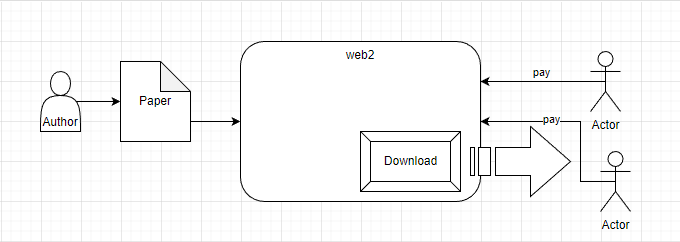
\includegraphics[width=3in]{assets/web2.png}
  \caption{User Pay for Download in Web2.0}
\end{figure}

Web2, also known as the social web, refers to the current state of the internet that we use today, which is primarily focused on social media, e-commerce, and other web-based applications that allow users to interact with each other and with content in various ways. In Web2, payment systems are typically centralized, meaning that they are controlled by a single entity or organization. For example, when we make a purchase on an e-commerce website, we typically use a centralized payment system like PayPal or a credit card. These systems rely on intermediaries to facilitate transactions, which can result in higher transaction fees and longer processing times.

Web3, also known as the decentralized web, represents a shift toward a more open, decentralized, and secure internet that is built on blockchain technology. In Web3, payment systems are decentralized, meaning that they are not controlled by a single entity or organization. Instead, payments are made using cryptocurrency, which is a digital asset that is secured by cryptographic techniques and operates independently of central banks and other financial institutions. Cryptocurrency payments are processed directly between users without the need for intermediaries, which can result in lower transaction fees and faster processing times.

Overall, the main difference in payment systems between Web2 and Web3 is the degree of centralization. Web2 payment systems are centralized, while Web3 payment systems are decentralized. While Web3 is still in its early stages, it has the potential to revolutionize the way we think about payments, transactions, and financial systems.


\begin{figure}[h]
  \centering
  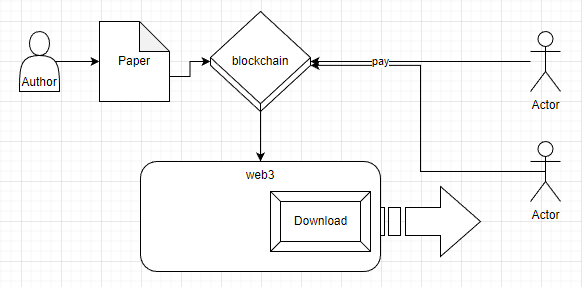
\includegraphics[width=3in]{assets/web3.png}
  \caption{User Pay for Download in Web3.0}
\end{figure}
  

\section{DAO to DeSci}


The DAO, or Decentralized Autonomous Organization, was a decentralized venture capital fund that operated on the Ethereum blockchain in 2016. It was created as a way to enable a group of individuals to pool their resources and invest in new projects without the need for a central authority or intermediary.

The DAO was essentially a smart contract on the Ethereum blockchain that contained a set of rules for how the organization would operate. Members could buy tokens that would give them voting rights to make decisions about which projects to invest in. Once a project was selected, the funds were automatically sent to the project's creators, and the project would be added to the DAO's portfolio.


\begin{figure}[h]
  \centering
  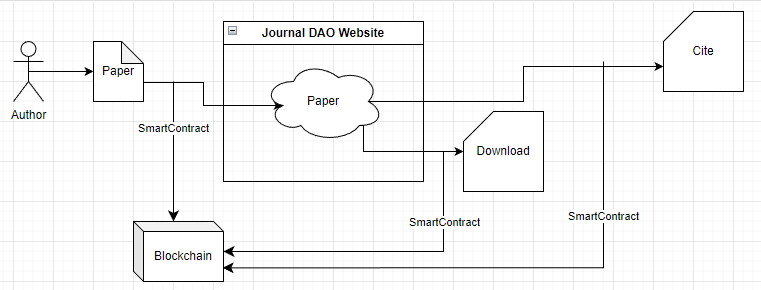
\includegraphics[width=3.2in]{assets/jdao.png}
  \caption{Journal DAO}
\end{figure}

However, the DAO was also susceptible to vulnerabilities, and in June 2016, a hacker exploited a vulnerability in the smart contract, stealing around "\$"50 million worth of Ethereum. This led to a contentious debate within the Ethereum community about how to handle the situation, and ultimately, a hard fork of the Ethereum blockchain was implemented to restore the stolen funds to their original owners.

Despite the controversy surrounding the DAO, it remains an important milestone in the development of blockchain technology, demonstrating the potential of decentralized autonomous organizations to enable new forms of collaboration and investment. Since then, there have been numerous other projects that have built on the DAO's ideas and sought to improve upon its flaws.

Since the DAO incident in 2016, the development of decentralized autonomous organizations (DAOs) has continued to evolve and expand, with new projects and platforms emerging to address the limitations of earlier attempts.

One of the most significant developments in recent years has been the emergence of DAO platforms that offer a more user-friendly and accessible way to create and manage decentralized organizations. These platforms provide tools and templates for creating DAOs, as well as built-in features such as voting, proposal submission, and fund management.

Some of the popular DAO platforms that have emerged in recent years include Aragon, MolochDAO, Colony, and DAOstack. These platforms enable anyone to create and participate in a decentralized organization, with a range of potential use cases such as investment funds, decentralized communities, and decentralized governance.


Another notable development in the DAO space has been the integration of blockchain technology with other emerging technologies, such as non-fungible tokens (NFTs) and decentralized finance (DeFi). For example, some DAOs are exploring the use of NFTs as a way to represent membership or ownership in the organization, while others are using DeFi protocols to manage and distribute funds.

Overall, the development of DAOs continues to evolve and mature, with new ideas and innovations emerging all the time. As blockchain technology and decentralized systems become more mainstream, it is likely that we will see an increasing number of DAOs being created and used for a variety of purposes.


\begin{figure}[h]
  \centering
  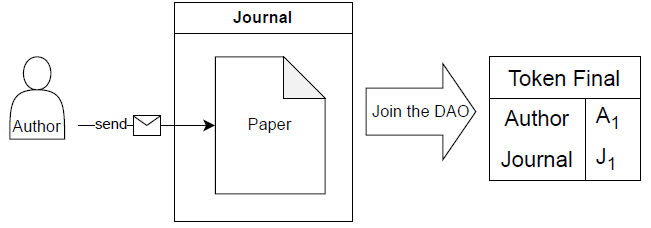
\includegraphics[width=3.2in]{assets/daopaper.png}
  \caption{Distribute Token by DAO}
\end{figure}


After the author publishes the paper in the Web3.0 journal, the paper is stored on a blockchain, afterthen TOKEN is distributed using the DAO framework.


\begin{figure}[h]
  \centering
  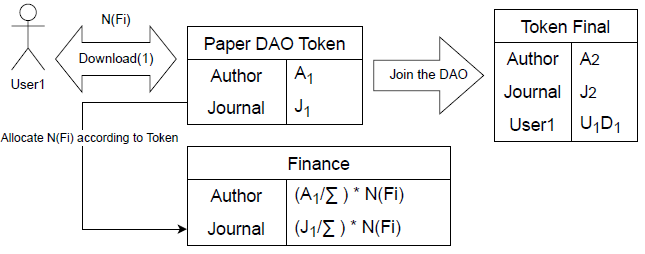
\includegraphics[width=3.2in]{assets/download1.png}
  \caption{Distribute Token while User Download}
\end{figure}


For example, someone downloading papers will creates finance.The funds received will be distributed to all holders in proportion to the token of the DAO framework. After that, users who download the paper will also receive a certain token and will be able to share the funds later. In other words, the user who download thie paper also becomes a holder and also own this paper.


\begin{figure}[h]
  \centering
  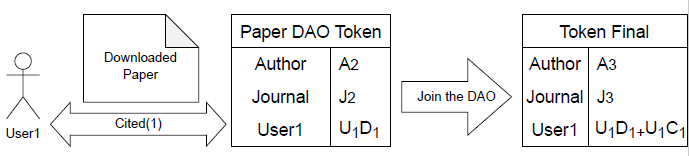
\includegraphics[width=3.2in]{assets/cite1.png}
  \caption{Distribute Token while User Cite Downloaded Paper}
\end{figure}


After downloading the paper, user can cite this paper in own paper and can get more token.


\begin{figure}[h]
  \centering
  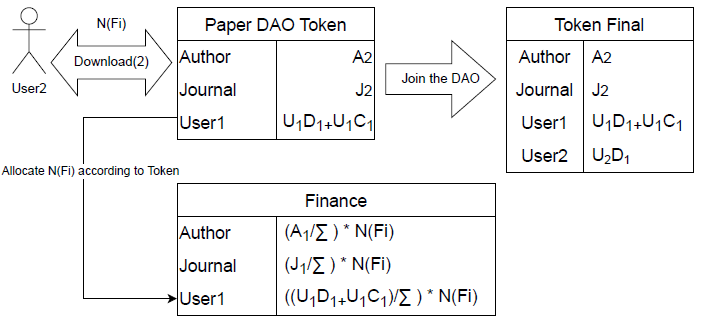
\includegraphics[width=3.2in]{assets/donwload2.png}
  \caption{Distribute Token while Another User Download}
\end{figure}


The currency paid by user2 when downloading the paper will continue to be distributed to all holders in proportion to the token. at this point, the holders already include user1. Both the author and the user who downloaded the paper will own the paper in proportion, and once the paper creates finance, it will be distributed to all owners.

\section{DeFi Deduced}

Defi deduced is a term that could be used to describe the process of applying deductive reasoning to the field of decentralized finance (defi). Deductive reasoning, or deduction, is making an inference based on widely accepted facts or premises. For example, one could deduce that a certain defi protocol is secure if it has been audited by a reputable firm and has no known vulnerabilities. Defi deduced could also refer to the outcome of such reasoning, such as a conclusion or a judgment about a defi project or phenomenon. For instance, one could deduce that the demand for defi services is increasing if the total value locked (TVL) in defi platforms is rising. Defi deduced could be seen as a way of applying logic and rigor to the analysis and evaluation of defi, which is a complex and dynamic domain that involves various aspects such as cryptography, economics, governance, and social behavior.


\section{Conclusion}
The conclusion goes here.


\section*{Acknowledgments}
This should be a simple paragraph before the References to thank those individuals and institutions who have supported your work on this article.



{\appendix[Proof of the Zonklar Equations]
Use $\backslash${\tt{appendix}} if you have a single appendix:
Do not use $\backslash${\tt{section}} anymore after $\backslash${\tt{appendix}}, only $\backslash${\tt{section*}}.
If you have multiple appendixes use $\backslash${\tt{appendices}} then use $\backslash${\tt{section}} to start each appendix.
You must declare a $\backslash${\tt{section}} before using any $\backslash${\tt{subsection}} or using $\backslash${\tt{label}} ($\backslash${\tt{appendices}} by itself
 starts a section numbered zero.)}



%{\appendices
%\section*{Proof of the First Zonklar Equation}
%Appendix one text goes here.
% You can choose not to have a title for an appendix if you want by leaving the argument blank
%\section*{Proof of the Second Zonklar Equation}
%Appendix two text goes here.}



\section{References Section}
You can use a bibliography generated by BibTeX as a .bbl file.
 BibTeX documentation can be easily obtained at:
 http://mirror.ctan.org/biblio/bibtex/contrib/doc/
 The IEEEtran BibTeX style support page is:
 http://www.michaelshell.org/tex/ieeetran/bibtex/
 
 % argument is your BibTeX string definitions and bibliography database(s)
%\bibliography{IEEEabrv,../bib/paper}
%
\section{Simple References}
You can manually copy in the resultant .bbl file and set second argument of $\backslash${\tt{begin}} to the number of references
 (used to reserve space for the reference number labels box).

\begin{thebibliography}{1}
\bibliographystyle{IEEEtran}

\bibitem{ref1}
{\it{Mathematics Into Type}}. American Mathematical Society. [Online]. Available: https://www.ams.org/arc/styleguide/mit-2.pdf

\bibitem{ref2}
T. W. Chaundy, P. R. Barrett and C. Batey, {\it{The Printing of Mathematics}}. London, U.K., Oxford Univ. Press, 1954.

\bibitem{ref3}
F. Mittelbach and M. Goossens, {\it{The \LaTeX Companion}}, 2nd ed. Boston, MA, USA: Pearson, 2004.

\bibitem{ref4}
G. Gr\"atzer, {\it{More Math Into LaTeX}}, New York, NY, USA: Springer, 2007.

\bibitem{ref5}M. Letourneau and J. W. Sharp, {\it{AMS-StyleGuide-online.pdf,}} American Mathematical Society, Providence, RI, USA, [Online]. Available: http://www.ams.org/arc/styleguide/index.html

\bibitem{ref6}
H. Sira-Ramirez, ``On the sliding mode control of nonlinear systems,'' \textit{Syst. Control Lett.}, vol. 19, pp. 303--312, 1992.

\bibitem{ref7}
A. Levant, ``Exact differentiation of signals with unbounded higher derivatives,''  in \textit{Proc. 45th IEEE Conf. Decis.
Control}, San Diego, CA, USA, 2006, pp. 5585--5590. DOI: 10.1109/CDC.2006.377165.

\bibitem{ref8}
M. Fliess, C. Join, and H. Sira-Ramirez, ``Non-linear estimation is easy,'' \textit{Int. J. Model., Ident. Control}, vol. 4, no. 1, pp. 12--27, 2008.

\bibitem{ref9}
R. Ortega, A. Astolfi, G. Bastin, and H. Rodriguez, ``Stabilization of food-chain systems using a port-controlled Hamiltonian description,'' in \textit{Proc. Amer. Control Conf.}, Chicago, IL, USA,
2000, pp. 2245--2249.

\end{thebibliography}


\newpage

\section{Biography Section}
If you have an EPS/PDF photo (graphicx package needed), extra braces are
 needed around the contents of the optional argument to biography to prevent
 the LaTeX parser from getting confused when it sees the complicated
 $\backslash${\tt{includegraphics}} command within an optional argument. (You can create
 your own custom macro containing the $\backslash${\tt{includegraphics}} command to make things
 simpler here.)
 
\vspace{11pt}

\bf{If you include a photo:}\vspace{-33pt}
\begin{IEEEbiography}[{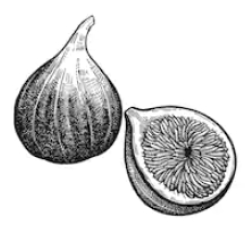
\includegraphics[width=1in,height=1.25in,clip,keepaspectratio]{fig1}}]{Michael Shell}
Use $\backslash${\tt{begin\{IEEEbiography\}}} and then for the 1st argument use $\backslash${\tt{includegraphics}} to declare and link the author photo.
Use the author name as the 3rd argument followed by the biography text.
\end{IEEEbiography}

\vspace{11pt}

\bf{If you will not include a photo:}\vspace{-33pt}
\begin{IEEEbiographynophoto}{John Doe}
Use $\backslash${\tt{begin\{IEEEbiographynophoto\}}} and the author name as the argument followed by the biography text.
\end{IEEEbiographynophoto}




\vfill

\end{document}


